% Fig. 1 source: rolling-horizon procedure with state carry-forward (conceptual, no data).
% Build: scripts/build_figures.sh  ->  manuscript/figures/fig_rolling.pdf
\documentclass[tikz,border=4pt]{standalone}
\usepackage[T1]{fontenc}
\usepackage{lmodern}
\usetikzlibrary{arrows.meta,decorations.pathreplacing}
\begin{document}
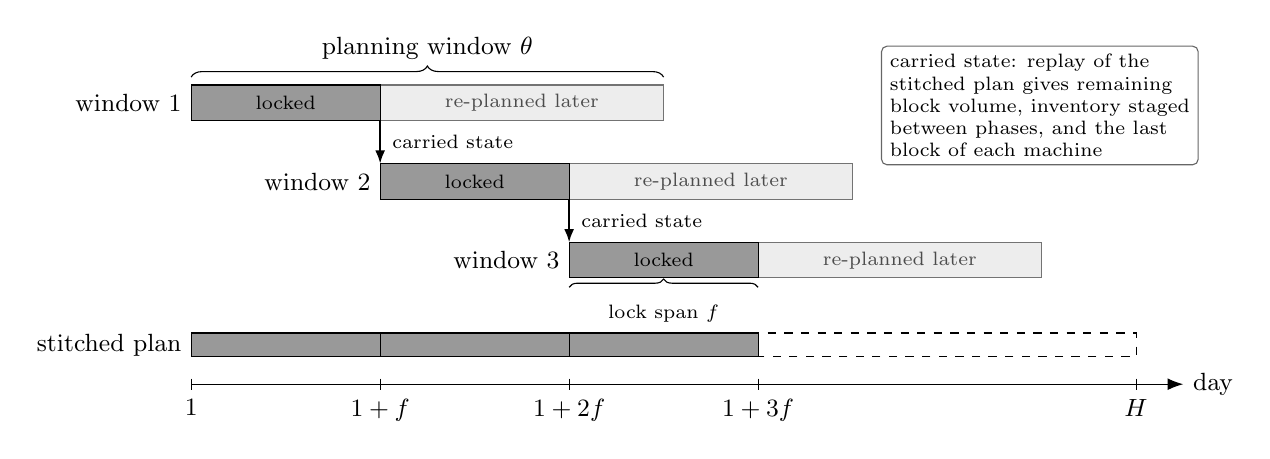
\begin{tikzpicture}[x=0.6cm,y=1cm,font=\small]
  \def\f{4}\def\th{10}
  % windows k = 1..3 starting at s = 0, f, 2f
  \foreach \k/\s/\y in {1/0/3, 2/4/2, 3/8/1} {
    \fill[black!7] (\s,\y) rectangle (\s+\th,\y+0.45);
    \draw[black!55] (\s,\y) rectangle (\s+\th,\y+0.45);
    \fill[black!40] (\s,\y) rectangle (\s+\f,\y+0.45);
    \draw (\s,\y) rectangle (\s+\f,\y+0.45);
    \node[font=\scriptsize] at (\s+\f/2,\y+0.225) {locked};
    \node[font=\scriptsize,black!70] at (\s+\f+3,\y+0.225) {re-planned later};
    \node[left] at (\s,\y+0.225) {window \k};
  }
  % carry-forward arrows from the end of each lock span to the start of the next window
  \foreach \s/\y in {4/3, 8/2} {
    \draw[-{Latex[length=1.7mm]},thick] (\s,\y) -- (\s,\y-0.55+0.0) ;
    \node[font=\scriptsize,anchor=west] at (\s+0.05,\y-0.27) {carried state};
  }
  % braces for theta and f
  \draw[decorate,decoration={brace,amplitude=4pt}] (0,3.55) -- (\th,3.55) node[midway,above=3pt] {planning window $\theta$};
  \draw[decorate,decoration={brace,amplitude=3pt,mirror}] (12,0.88) -- (8,0.88);
  \node[font=\scriptsize,below] at (10,0.78) {lock span $f$};
  % stitched plan
  \foreach \s in {0,4,8} {\fill[black!40] (\s,0) rectangle (\s+\f,0.3); \draw (\s,0) rectangle (\s+\f,0.3);}
  \draw[dashed] (12,0) rectangle (20,0.3);
  \node[left] at (0,0.15) {stitched plan};
  % axis
  \draw[-{Latex[length=2mm]}] (0,-0.35) -- (21,-0.35) node[right] {day};
  \foreach \x/\l in {0/1, 4/{$1+f$}, 8/{$1+2f$}, 12/{$1+3f$}, 20/{$H$}}
    \draw (\x,-0.28) -- (\x,-0.42) node[below] {\l};
  % legend for carried state
  \node[draw=black!60,rounded corners=2pt,font=\scriptsize,align=left,anchor=north west,inner sep=3pt]
    at (14.6,3.95) {carried state: replay of the\\stitched plan gives remaining\\block volume, inventory staged\\between phases, and the last\\block of each machine};
\end{tikzpicture}
\end{document}
